


\documentclass{article}
\usepackage{graphicx}
\graphicspath{ {/home/tk_conda/Documents/Shoriya/HIWI/RTS_documents/texdoc} }
\usepackage{listings}
\usepackage{color}

\definecolor{dkgreen}{rgb}{0,0.6,0}
\definecolor{gray}{rgb}{0.5,0.5,0.5}
\definecolor{mauve}{rgb}{0.58,0,0.82}

\lstset{frame=tb,
  language=C,
  aboveskip=3mm,
  belowskip=3mm,
  showstringspaces=false,
  columns=flexible,
  basicstyle={\small\ttfamily},
  numbers=none,
  numberstyle=\tiny\color{gray},
  keywordstyle=\color{blue},
  commentstyle=\color{dkgreen},
  stringstyle=\color{mauve},
  breaklines=true,
  breakatwhitespace=true,
  tabsize=3
}

\usepackage{tikz}
\usetikzlibrary{arrows,calc,positioning,shadows,shapes}

\begin{document}
	\begin{center}
		\thispagestyle{empty}
		\parskip=14pt%
		\vspace*{3\parskip}%
		
		\large Real Time System Department
				\\
		Fog Computing of Self Balancing Robot
				
		
		
		By
		
		(Shoriya Chauhan)
		
		
		
		Under the supervision of
		\\
		MSc. Alexandre Venito
		\\
		Prof. Gerhard Fohler
		\\
		\rule{7cm}{0.4pt}\\
		
				
		
		
		
		(8th May 2020)
	\end{center}
	\newpage
	


 	\section{Motivation}
 	Improvment for the next generation industry is the key idea to implement this project.The traditional robots have dedicated controller and resources to meet the real tme constraints.The main idea here is to be able to do complex funcitonality on fog node meeting the real time contraints, which can not be done via dedicated controller and resourses.Fog computing may provide local data processing along with real time communicatioon mechanism.
 	
 	\section{Project Flow}
	Here we are implemneting a self balancing robot running on esp32 and the main PID control loop to be implemented on the fog node while meeting the requirement of the robot to be balanced. 
	\\
	Flow of the project:
	\begin{itemize}
	\item To understand the communication protocol of the lego sensors
	\item Implement communication of lego sensors with Arduino
	\item Integrate the sensors togther to build self balaning bot
	\item Change from Arduino to esp32 for the wireless communication
	\item Structure the robot
	\item Get exact value of the PID
	\item Shift the PID function on fog node. 
	 \end{itemize}	
	 
	\section{Literature Survey}
	Consider broomstick on the index finger, when trying to balance it we will have to move the finger in direction of the falling broomstick. Similarly the robot would fall either forward or backward which can be controlled by moving the robot either backward or forward.
	To make a balancing robot we need to control the center of gravity of the robot just at the pivot point. 
	\subsection{Requirement for balancing the robot}	
	\begin{itemize}
		\item Direction the robot is falling 
		\item Robot tilts
	\end{itemize}	
	These information can be dedSelfBalancing Robotuced from the accelero-meter and gyroscope in a complimentary filter.
	
	\begin{figure}[h]
		\centering
		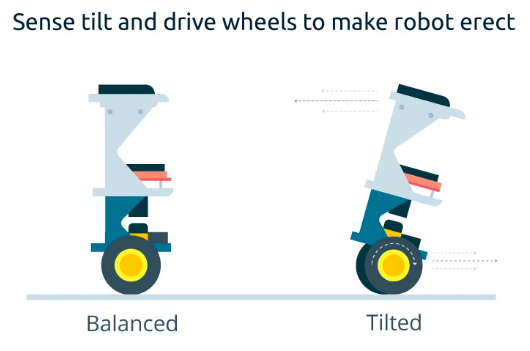
\includegraphics[width=100mm,scale=0.5]{balance.png}
		\caption{Tilt Angle and Balance}
		\label{Tilt Angle and Balance}
	\end{figure}

\pagebreak
	\section{Hardware required}
	 \begin{itemize}
	 	\item Lego Motors   
	 	\item Lego Gyroscopic Sensor  (replaced it with MPU6050)
	 	\item MPU6050
	 	\item Ultrasonic Sensor
	 	\item Arduino Mega 2560
	 	\item L298N H bridge
	 	\item ESP32
	 \end{itemize}
 	
 		\begin{table}[h]
 		\begin{center}
 			\caption{Sensors}
 			\label{tab:table1}
 			\begin{tabular}{l|c|r} % <-- Alignments: 1st column left, 2nd middle and 3rd right, with vertical lines in between
 				\textbf{Sensors} & \textbf{Output} & \textbf{Unit}\\
 				\hline
 				Rotary Encoder & Angle & deg\\
 				Ultrasonic Sensor & Distance & cm\\
 				Gyro Sensor & Angular Velocity & deg/sec\\
 			\end{tabular}
 		\end{center}
 		
 	\end{table}
 	
 	
 	
 	\subsection{Lego Motors}
 	Lego smart motor has built in encoders that can be used to make the robot move around in a very precise manner. It has a resolution of 360 counts per revolution which means it counts 360 when the robot completes one wheel rotation.
 	 
 	\begin{figure}[h]
 		\centering
 		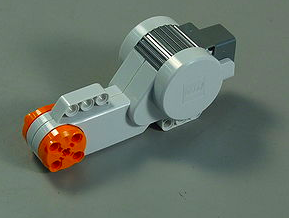
\includegraphics[width=50mm,scale=0.5]{legomotor}
 		\caption{LEGO MOTOR}
 		\label{ LEGO MOTOR}
 	\end{figure} 
  
 
 	\subparagraph{What are encoders used for?}
 	Encoders convert mechanical motion into electronic signal. By reading the encoder signals, the Arduino can figure out in which direction is the wheel turning and how many degrees.
 	
 	\subsection{Gyroscopic Sensor}
 	Gyro offset and Gyro drift have major impact on balancing the robot.
 	Gyro offset is the output when the gyro sensor does not rotate. In our case the gyro offset is 17. Gyro drift is time variation of gyro offset.
 	
 	 	
 	\subsection {MPU 6050}
 	The MPU 6050 is a 6 DOF (degrees of freedom) or a six-axis IMU sensor, which means that it gives six values as output: three values from the accelerometer and three from the gyroscope. The MPU 6050 is a sensor based on MEMS (micro electro mechanical systems) technology.
 	
 	\begin{figure}[h]
 		\centering
 		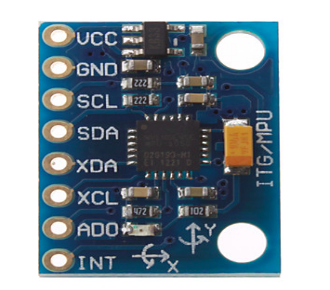
\includegraphics[width=50mm,scale=0.5]{mpu6050}
 		\caption{MPU6050}
 		\label{ MPU6050}
 	\end{figure}
 	
 	 	
 	\pagebreak
 	 
 	\subsection{Ultrasonic Sensor}
 	Ultrasonic sensor here is used to avoid obstacle. The robot would rotate itself when it senses an obstacle within 20 cm. It is done by rotating one wheel faster than the other. 
 	
 	\begin{figure}[h]
 		\centering
 		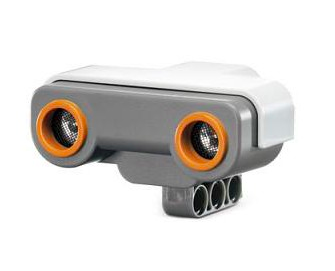
\includegraphics[width=50mm,scale=0.5]{ultrasonic}
 		\caption{Ultrasonic Sensor}
 		\label{ Ultrasonic Sensor}
 	\end{figure}
 
 	\subsection{L298N}
 	The L298 is an integrated monolithic circuit in a 15-lead Multiwatt and PowerSO20 packages. It is a high voltage, high current dual full bridge driver designed to accept standard TTL logic levels and drive inductive loads such as relays, solenoids, DC and stepping motors. 
 	
 	\begin{figure}[h]
 		\centering
 		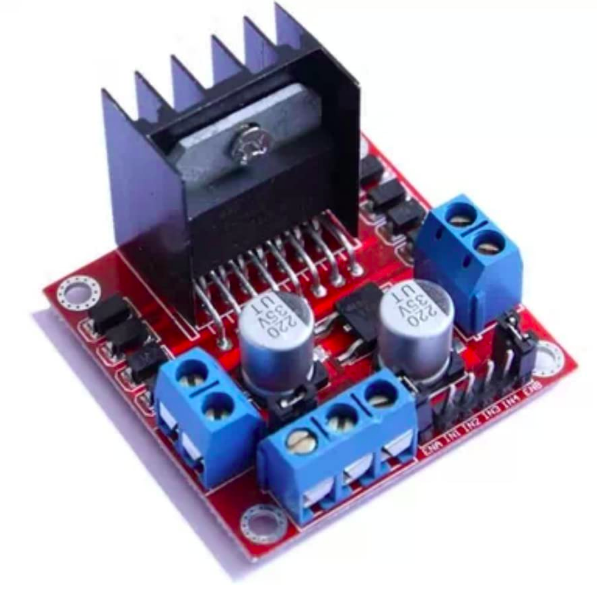
\includegraphics[width=50mm,scale=0.5]{L298N}
 		\caption{L298N H-Bridge}
 		\label{L298N H-Bridge}
 	\end{figure}
 
 	\pagebreak
 	
 	\section{Control System}
 	
 	To keep the robot balanced, the motors must counteract the robot falling. This action requires feedback and correcting elements. The feedback element is the MPU6050 gyroscope + accelerometer, which gives both acceleration and rotation in all three axes. The Arduino uses this to know the current orientation of the robot. The correcting element is the motor and wheel combination. 
 	
 	\subsection{Angle Measurement using MPU6050}
 	Gyroscopic sensor was replaced by MPU 6050 as it has both gyro meter and the accelero-meter therefore, it is easily to calculated the angle of inclination accurately using the complimentary filter. 
 	
 	The accelerometer can measure the force of the gravity, and with that information we can obtain the angle of the robot, the problem of the accelerometer is that it can also measure the rest of the forces the vehicle is someted, so it has lot of error and noise. The gyroscope measure the angular velocity, so if we integrate this measure we can obtain the angle the robot is moved, the problem of this measure is that is not perfect and the integration has a deviation, that means that in short time the measure is so good, but for long time terms the angle will deviate much form the real angle.

Those problems can be resolved be the combination of both sensors, that's called sensor fusion, and there are a lot of methods to combine it. 
 	
 	\subsection{Complimentary Filter}
 	Complimentary filter used to enhance the quality of accelerometer and gyroscope to give a define angle of inclination.
 	
 	\begin{figure}[h]
 		\centering
 		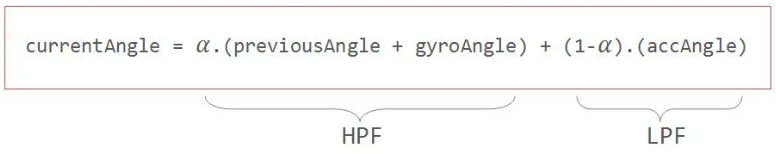
\includegraphics[width=100mm,scale=0.5]{complimentaryfilter}
 		\caption{Complimentary Filter}
 		\label{Complimentary Filter}
 	\end{figure}
 	
 	The measurement from accelerometer gets affected by sudden horizontal movements and the measurement from gyroscope gradually drifts away from actual value. In other words, the accelerometer reading gets affected by short duration signals and the gyroscope reading by long duration signals. These readings are, in a way, complementary to each other. Combine them both using a Complementary Filter and we get a stable, accurate measurement of the angle. The complementary filter is essentially a high pass filter acting on the gyroscope and a low pass filter acting on the accelerometer to filter out the drift and noise from the measurement.
 	
 	\textbf{currentAngle = 0.9934 * (previousAngle + gyroAngle) + 0.0066 * (accAngle)}
 	
 	0.9934 and 0.0066 are filter coefficients for a filter time constant of 0.75s. The low pass filter allows any signal longer than this duration to pass through it and the high pass filter allows any signal shorter than this duration to pass through. The response of the filter can be tweaked by picking the correct time constant. Lowering the time constant will allow more horizontal acceleration to pass through.
 	
 	\subsection{PID Controller}
 	
 	PID stands for Proportional, Integral and Derivative. In this algorithm, the error signal received is the input. And the following equation is applied onto the error signal
 	
 	
 	\begin{figure}[h]
 		\centering
 		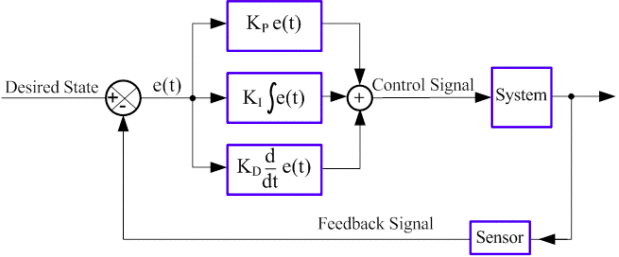
\includegraphics[width=100mm,scale=0.5]{PIDcontrol}
 		\caption{PID Controller}
 		\label{ PID Controller}
 	\end{figure}
 	
 	The proportional term (gain) makes a change to the output that is proportional to the current error value. Larger values typically mean faster response since the larger the error, the larger the Proportional term correction signal. However, an excessively large proportional gain will lead to instability and oscillation.
 	The Integral term is proportional to the amount of time the error is present. The integral term accelerates the movement of the process towards the set value and eliminates any residual steady-state error that occurs with a proportional only controller. The contribution from the integral term is dependent both on the magnitude of the error and on the duration of the error.
 	With the derivative term, the controller output is proportional to the rate of change of the measurement or error. The derivative term slows the rate of change of the controller output, most notably near the controller set value. It therefore reduces the magnitude of the overshoot produced by the integral component and improves stability. Larger Kd values decrease overshoot, but slows down transient response and may lead to instability from signal noise amplification from differentiation of the error.\\	
 		
 	
	\pagebreak
 
 	\textbf{TUNING a PID controller}
 	
 	Tuning: A good Control System will have low rise time, settling time, peak overshoot and steady state error. Therefore, the Kp, Kd, Ki need to be finely tuned to adjust the contribution of the above factors in order to acquire a good Control System.
 	
 	\begin{itemize}
 	\item SetKp=Ki=Kd= 0.
 	\item Adjust Kp until the system remains in balance, but rapidly oscillates around equilibrium.
 	\item Adjust Kd until the system reaches steady state.•If there is a steady state error, tune Ki. However, be warned that if the system is not actually reaching equilibrium, the integral term can dominate the controller and otherwise have negative effects on your controller.
 	\end{itemize}
 
  
  \section{Integrating ESP32}
  ESP32 is higly integrated solution for IoT Applications with bluetooth, WiFi. Esp32 uses I2C commmunication to communicate with mpu6050.
  \\  
  Pin Connections for self balancing robot 
  \begin{itemize}
  	\item MPU connection:
  		\\
		SDA 21 -- Pin3
		\\	
		SCL 22 -- Pin4
		\\ 	  
		\item Motor Connection
		\\
			\begin{figure}[h]
 			\centering
 			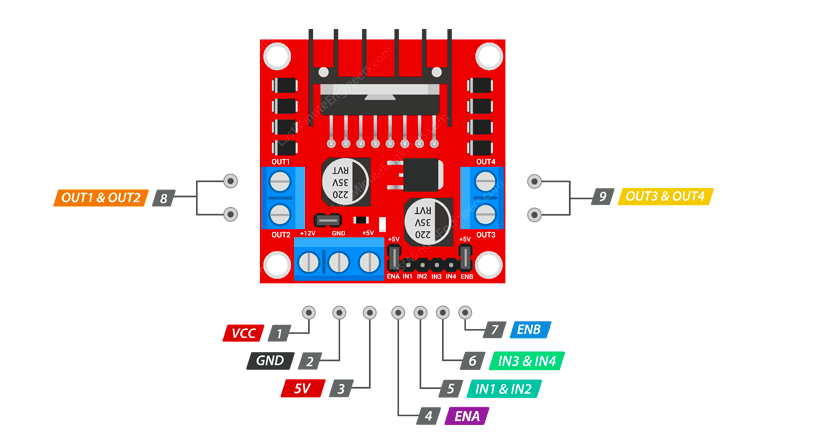
\includegraphics[width=100mm,scale=0.5]{PinConnection}
 			\caption{Motor Connector}
 			\label{Pin Specification for L298N H-Bridge }
 		\end{figure}
 	
 		VCC	-- Battery 9V\\
 		GND	-- GND Battery\\
 		5V	-- 5V ESP32\\
 		\\
 		ENA -- 12\\
 		ENB -- 14\\
 		IN1	-- 26\\
 		IN2	-- 27\\
 		IN3	-- 18\\
 		IN4	-- 19\\
		
 		OUT1 -- Motor Connector AN IN\\
 		OUT2 -- Motor Connector GND\\
 		OUT3 -- Motor Connector AN IN\\
 		OUT4 -- Motor Connector GND
	\end{itemize}
  
  \section{Structure Modelling}
  The struture is so built that it tries to divides it weight equally and the center of mass is maintained. The base layer hols the L298N motor control and the esp32 and the top is where the mpu6050 is standing verticially. And integrating two batteries one for esp32 and other for L298N motor controller.
  
  	\begin{figure}[h]
 			\centering
 			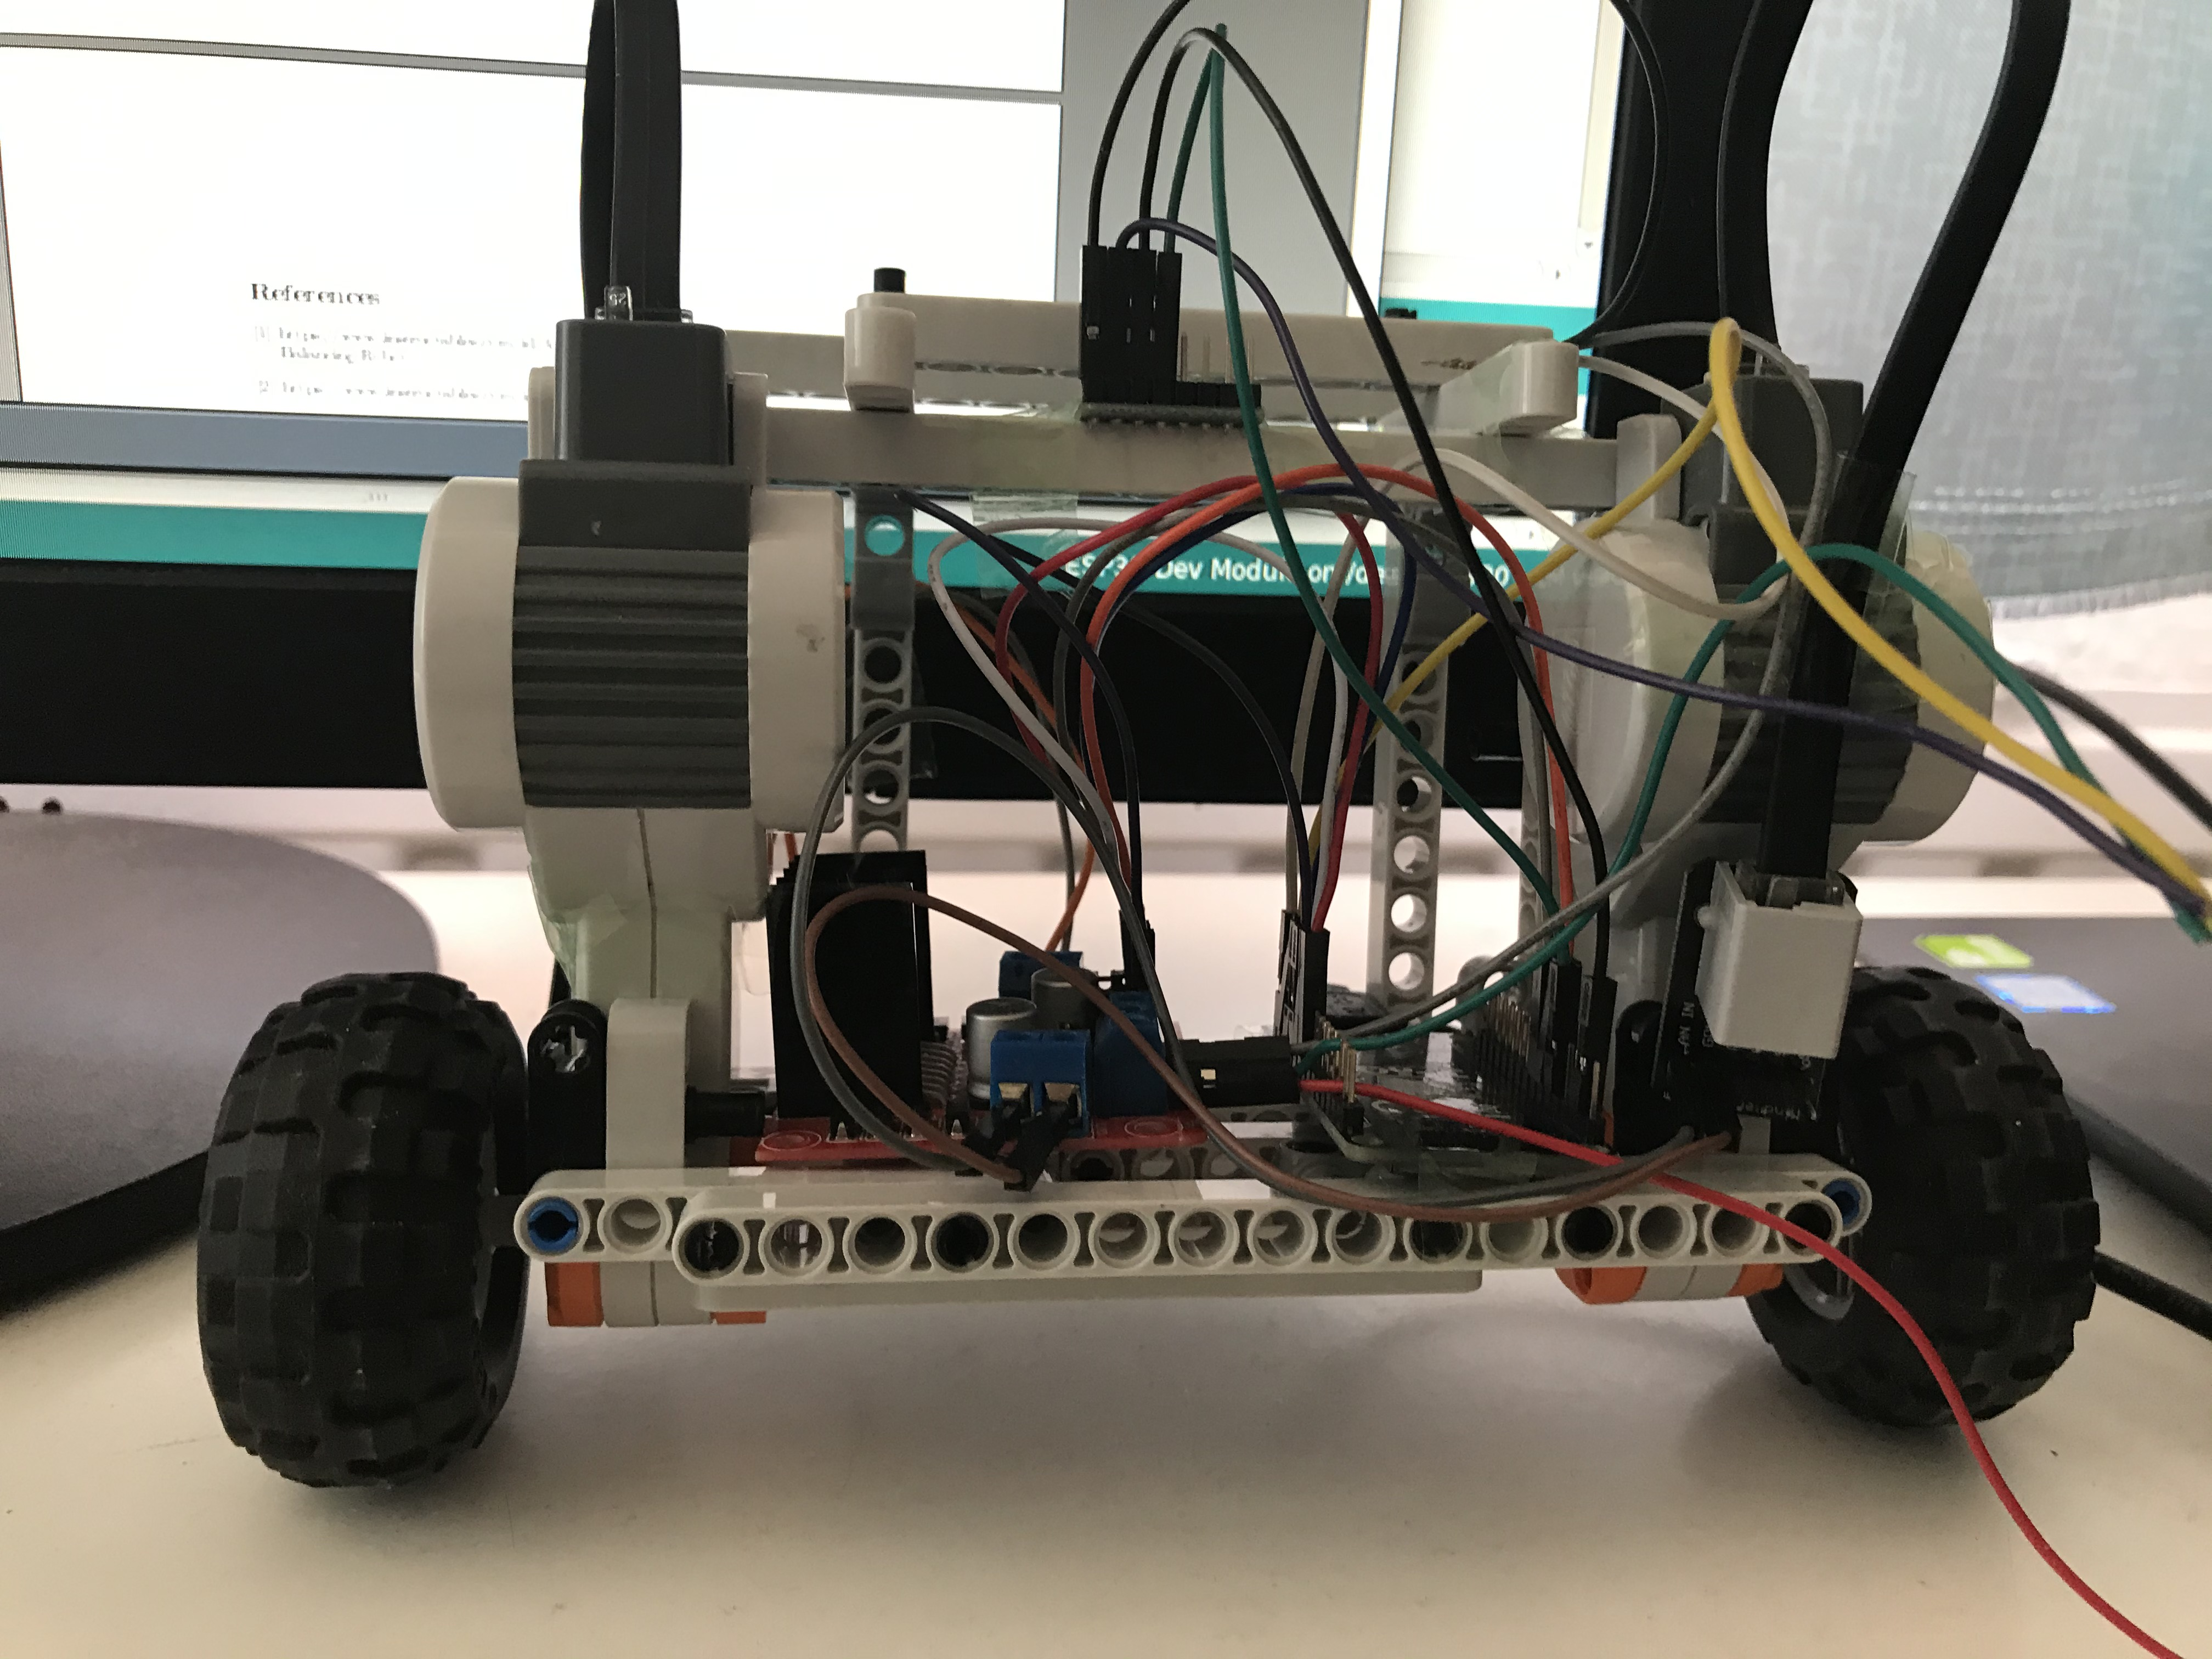
\includegraphics[width=100mm,scale=0.5]{Structure}
 			\caption{Structure}
 			\label{Structure }
 		\end{figure}
 		
 	The struture is able to balance it self with the defined values of PID when the PId is implemented on the controller.
  
  \section{Fog Node}
  Here we using Python socket as our server node (fog node) to implement PID module. The esp32 functions to supply the current angle and the server replies back with the change in motor to be stable. 
  With fog computing technology, all the processing happens on devices physically closer to where the data is collected, instead of sending data to the cloud.
  
  \subsection{Exeution time}
  
     The first the foremost step was to find the maximum delay that the robot can withstand to still be balanced.This is done by using the millis() or micros() function in Arduino to find the approximate execution time of the program in loop. 
     We find that it takes around 1ms for the code to run and the robot to still be balanced. To this we added a delay funtion to find the minimum number of gyroscope value required in a time frame for it to be balanced.
     A delay of 20ms was fair enough for the bot to still be balanced with Kp value to be 280. 
     \begin{lstlisting}
		void loop() {
  			startTime =millis();
				//Code for Angle Calculations
				//Code for PID Funtion  
  			delay(20);
  			Serial.println(millis()-startTime);
  
		}
		\end{lstlisting}
       
	And after shifting the PID code to the python server the total execution time on ESP32 was re-calculated. It takes around 2050 ms to get the motor speed and the turning direction. 

  	\tikzstyle{line} = [draw, -latex']

\tikzset{label/.style={draw=gray, ultra thin, rounded corners=.25ex, fill=gray!20,text width=4cm, text badly centered,  inner sep=2ex, anchor=east, minimum height=4em}}

\begin{figure}[!htb]
\centering
\resizebox{\textwidth}{!}{%
\begin{tikzpicture}[node distance=5cm,auto,>=latex']
% Place nodes
\node [label] (init) {Angle Calculations from MPU6050};
\node [label, right of=init] (node) {Convert Angle to String};
\node [label, right of=node] (node1) {Send Angle to Server};
\node [label, right of=node1] (node2) {Convert String to Float};
\node [label, right of=node2] (node3) {PID Calculation};
\node [label, right of=node3] (node4) {Send Motor speed Value to ESP32};

% Draw edges
\path [line] (init) -- (node);
\path [line] (node) -- (node1);
\path [line] (node1) -- (node2);
\path [line] (node2) -- (node3);
\path [line] (node3) -- (node4);

\end{tikzpicture}
}
\caption{Loop Execution}
\label{fig:dummy}
\end {figure}

We have to reduce the the communication time from the esp32 to the fog node and back. Here we introduce OPC-UA (Open Platform Communication United Architecture) which is a data exchange standard for next generation industrial communication

  \pagebreak
  \section{Open Platform Communication United Architecture-OPC-UA}
  OPC-UA is a mechanism for transferring information between server and client which is secure,open and reliable. 
	Here, we will implement the OPC-UA fog server for calculating the PID function and the esp32 will act like an OPC-UA client. 
	
	\subsection{Steps invloved in configuration of OPC UA}
	\begin{itemize}
	\item Server Initial Configuration
	\item Local Discovery Server LDS - Registration 
	\item Client Configuration
	\item Local Discovery Server LDS - Discovery 
	\item Connection configuration
	 \end{itemize}	
	 
	\subsection{Steps invloved in configuration of OPC UA}
	  	
  	 
  \pagebreak
  \section{Problems faced}
  Problem : Lego Ultrasonic sensor does use simple I2C communication\\
  Solution : Used Separate library for re-start frame I2C communication with arduino\\
  
  Problem : Either the MPU6050 worked or the Motor- Due to separate ground\\
  Solution : It is necessary when there are groups of circuit need to interface with each other and ground is the reference. \\
  
  Problem : Shifting code from arduino to ESP32\\
  Solution : ESP32 is not compatible with the libraries for MPU6050 and I2C used in arduino. Hence the code had to be modified for specific integration of gyroscope and accelerometer.\\
    
  Problem : Getting exact value of the Kp,Ki and Kd
  Solution : Have to change the Target angle as well as the Kp Ki Kd value on trial and error to get the exact value for the balance
    	
 	\pagebreak
 	\begin{thebibliography}{9}
 		\bibitem{Instrutable} 
 		{https://www.instructables.com/id/Arduino-Self-Balancing-Robot-1/}{self-Balancing Robot}
 		
 		\bibitem{Instrutable} 
 		{https://www.instructables.com/id/Self-Balancing-Robot-1/}
 		
 		\bibitem{osoyoo} 
 		{https://osoyoo.com/2018/08/08/self-balancing-robot-pid-control/}
 		
 		\bibitem{pdf} 
 		{https://www.cs.cmu.edu/~16311}
 		 
 		 \bibitem{L298N} 
 		 {https://howtomechatronics.com/tutorials/arduino/arduino-dc-motor-control-tutorial-l298n-pwm-h-bridge/}
 		
 		
 	\end{thebibliography}
 	
\end{document}

